\chapter{Metodología y herramientas}
\section{Definición de la metodología aplicada}

Desde el principio se definieron cinco fases principales:

\begin{itemize}
    \item Reuniones iniciales.
    \item Búsqueda de información.
    \item Formación y entrenamiento de la nariz electrónica (e\nobreakdash-nose).
    \item Pruebas comparativas con los agentes caninos.
    \item Redacción final de la documentación.
\end{itemize}

Sin embargo, el contenido específico, la secuencia detallada y la carga de trabajo dentro de cada fase no podían fijarse de antemano, ya que dependen de la disponibilidad de recursos, de las personas implicadas y de la información que se vaya obteniendo durante el avance del proyecto. Por este motivo se adoptó un enfoque ligero, apoyado en metodologías ágiles (Scrum y Kanban), que facilita mantener un ritmo constante y una alta capacidad de adaptación ante cambios y necesidades emergentes.

\subsubsection{Control de versiones con Git}
Para garantizar la trazabilidad y poder revertir cambios si fuera necesario, se utiliza Git como sistema de control de versiones. Esto permite mantener un historial detallado de todas las modificaciones realizadas en el código y la documentación, facilitando la colaboración y la gestión del proyecto.
\par

Esto se logra a traves de un repositorio privado en GitHub gestionado mediante ramas, en el que se almacena todo el código fuente, documentación, información recopilada a modo de apuntes y recursos relacionados con el proyecto.

\subsubsection{Sprints adaptativos}
Se define como sprint a cada una de las fases anteriormente mencionadas. La duración de cada sprint se fija en funcion de una estimación del tiempo que se cree necesario para lograr los objetivos establecidos para esa fase.
\par

Antes de que inicie cada sprint (En los ultimos días del sprint anterior), se hace una organiacación aproximada de las tareas a realizar. Al comenzar el sprint, se hace una planificación más detallada de las tareas a realizar, asignando prioridades y fijando fechas de las posibles reuniones con los implicados. Durante el sprint, se revisa periódicamente el progreso y se ajustan las tareas y prioridades según sea necesario.

\subsubsection{Github Projects y Tablero Kanban}

Para la gestión de tareas, sprints y el seguimiento del progreso del proyecto, se utiliza GitHub Projects (En el repositorio anteriormente mencionado), que cuenta con un tablero Kanban integrado, como el que se muestra en la Figura~\ref{fig:tablero_kanban}. Este tablero permite visualizar las tareas en diferentes estados (Backlog, Ready, In progress, Done) y facilita la organización y priorización de las actividades. Cada tarea se representa como una tarjeta que puede moverse entre las columnas según su estado actual, proporcionando una visión clara del avance del proyecto.

\begin{figure}[H]
    \centering
    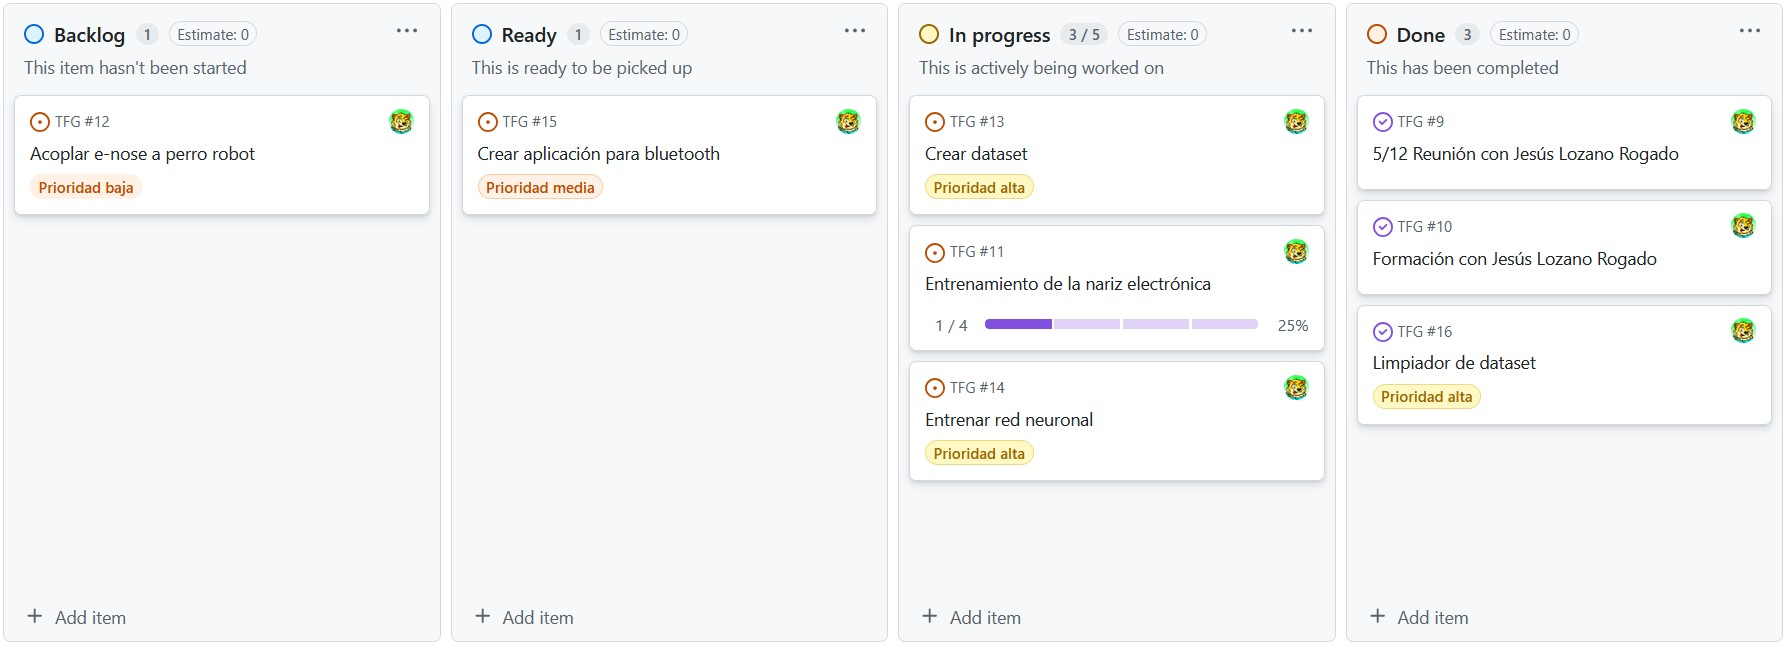
\includegraphics[width=0.9\textwidth]{pictures/Tablero_Kanban.jpg}
    \caption{Tablero Kanban del segundo sprint.}\label{fig:tablero_kanban}
\end{figure}

\subsection{Planificación}

\section{Herramientas utilizadas}
Dada la naturaleza del proyecto, es posible dsitinguir entre dos tipos de herramientas: herramientas hardware y herramientas software.

\subsection{Herramientas hardware}
Aquí se encuentra la principal herramienta para este estudio: la nariz electrónica utilizada para la toma de datos de las ditintas muestras y, posteriormente, para la realización de las pruebas con la ANN y la neuva aplicación móvil. Esta nariz electrónica ha sido diseñada y construida en el laboratorio de sensores de la Escuela de Ingenierías Industriales de Badajoz por Cristina Brugera Salas, bajo la supervisión del Dr.\ Jesús Lozano Rogado, cotutor de este trabajo.
\par

\begin{figure}[H]
    \centering
    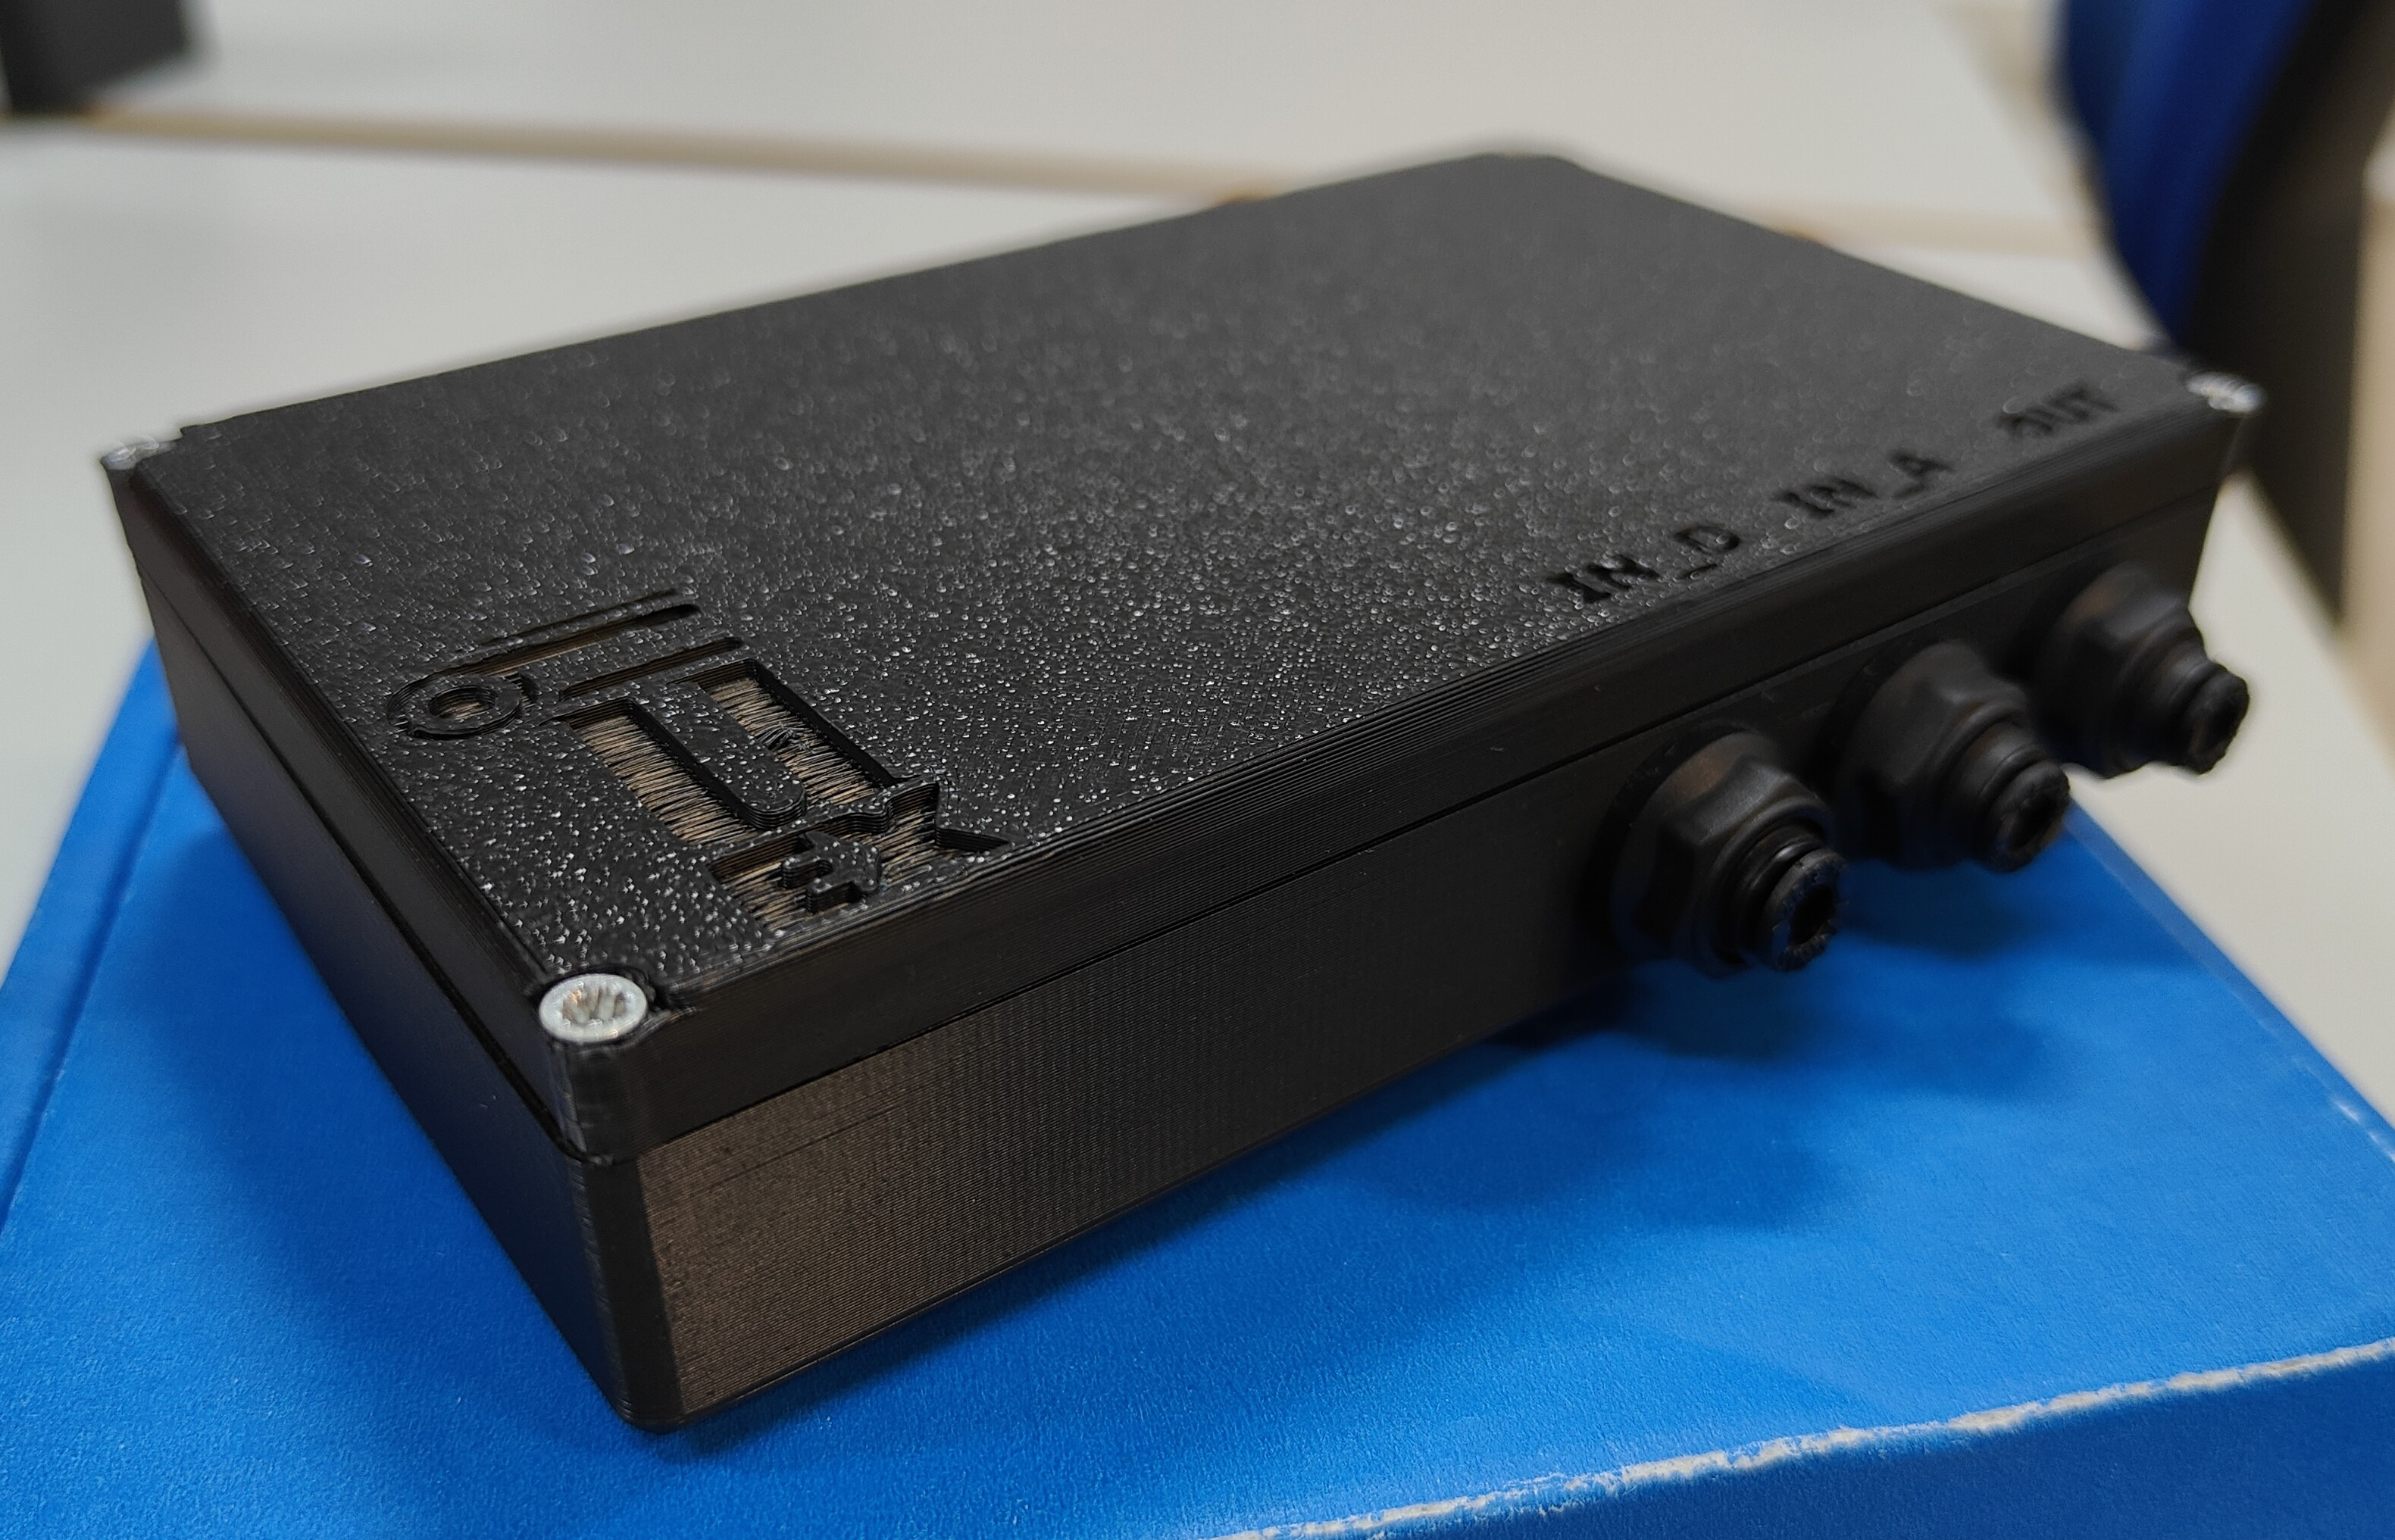
\includegraphics[width=0.7\textwidth]{pictures/Nariz_electronica.jpg}
    \caption{Carcasa de la nariz electrónica.}\label{fig:nariz_electronica}
\end{figure}

En la Figura~\ref{fig:nariz_electronica} se puede observar dicha nariz electrónica desde una vista exterior (La carcasa), donde están los orificios de entrada y salida de aire. La ``verdadera'' nariz electrónica es una placa PCB, diseñada y programada en el laboratorio de sensores de la Esuela de Ingenierias Industriales de Badajoz, que se encuentra en el interior de la carcasa. En esta placa es donde se encuentran los sensores de gases y el microcontrolador PIC32MM0256GPM048, además de contar con un módulo Bluetooth Rn4871 para la comunicación con una aplicación movil que la controla, y una entrada microUSB para poder conectarla a la corriente y cargar la bateria con la que cuenta. Toda esta placa se muestra en la Figura~\ref{fig:placa_pcb}.
\par

\begin{figure}[H]
    \centering
    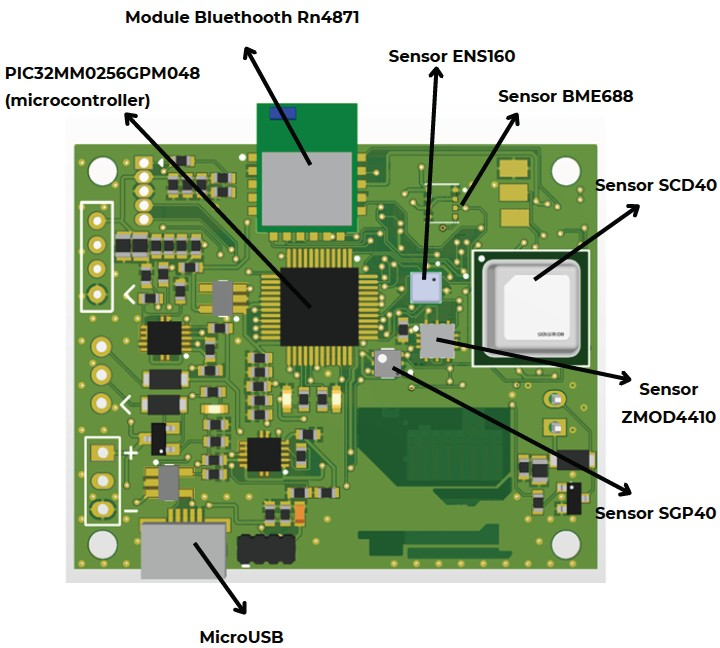
\includegraphics[width=0.7\textwidth]{pictures/Placa_PCB.jpg}
    \caption{Placa PCB de la nariz electrónica.}\label{fig:placa_pcb}
\end{figure}

El conjunto de sensores que componen esta nariz electrónica es el siguiente:
\begin{itemize}
    \item \textbf{SCD40} (PA): Sensor de CO$_2$, temperatura y humedad, fabricado por Sensirion.
    \item \textbf{SGP40} (MOS): Sensor de COV, fabricado por Sensirion.
    \item \textbf{BME688} (MOS): Sensor de presión, temperatura, humedad, COV, VSC y gas, fabricado por Bosch.
    \item \textbf{ENS160} (MOS): Sensor de COV, calidad del aire, VOX y NO$_2$, fabricado por ScioSense.
    \item \textbf{ZMOD4410} (MOS): Sensor de COV y CO$_2$, fabricado por Renesas.
\end{itemize}
\subsection{Herramientas software}

\subsubsection{Toma de muestras}
Para la fase de toma de muestras, en conjunto con la nariz electrónica mencionada en el apartado anterior, se ha utilzado una aplicación móvil desarrollada también por Cristina Brugera Salas, que permite controlar la nariz electrónica a través de Bluetooth, enviando comandos a través de la aplicación, y recoger los datos obtenidos por los sensores. Esta aplicación facilita la configuración de los parámetros de medición, el inicio y la detención de las pruebas, así como el almacenamiento y exportación de los datos recopilados para su posterior análisis. En la Figura~\ref{fig:app_toma_muestras} se muestra una captura de pantalla de la interfaz de la aplicación móvil mencionada.

\begin{figure}[H]
    \centering
    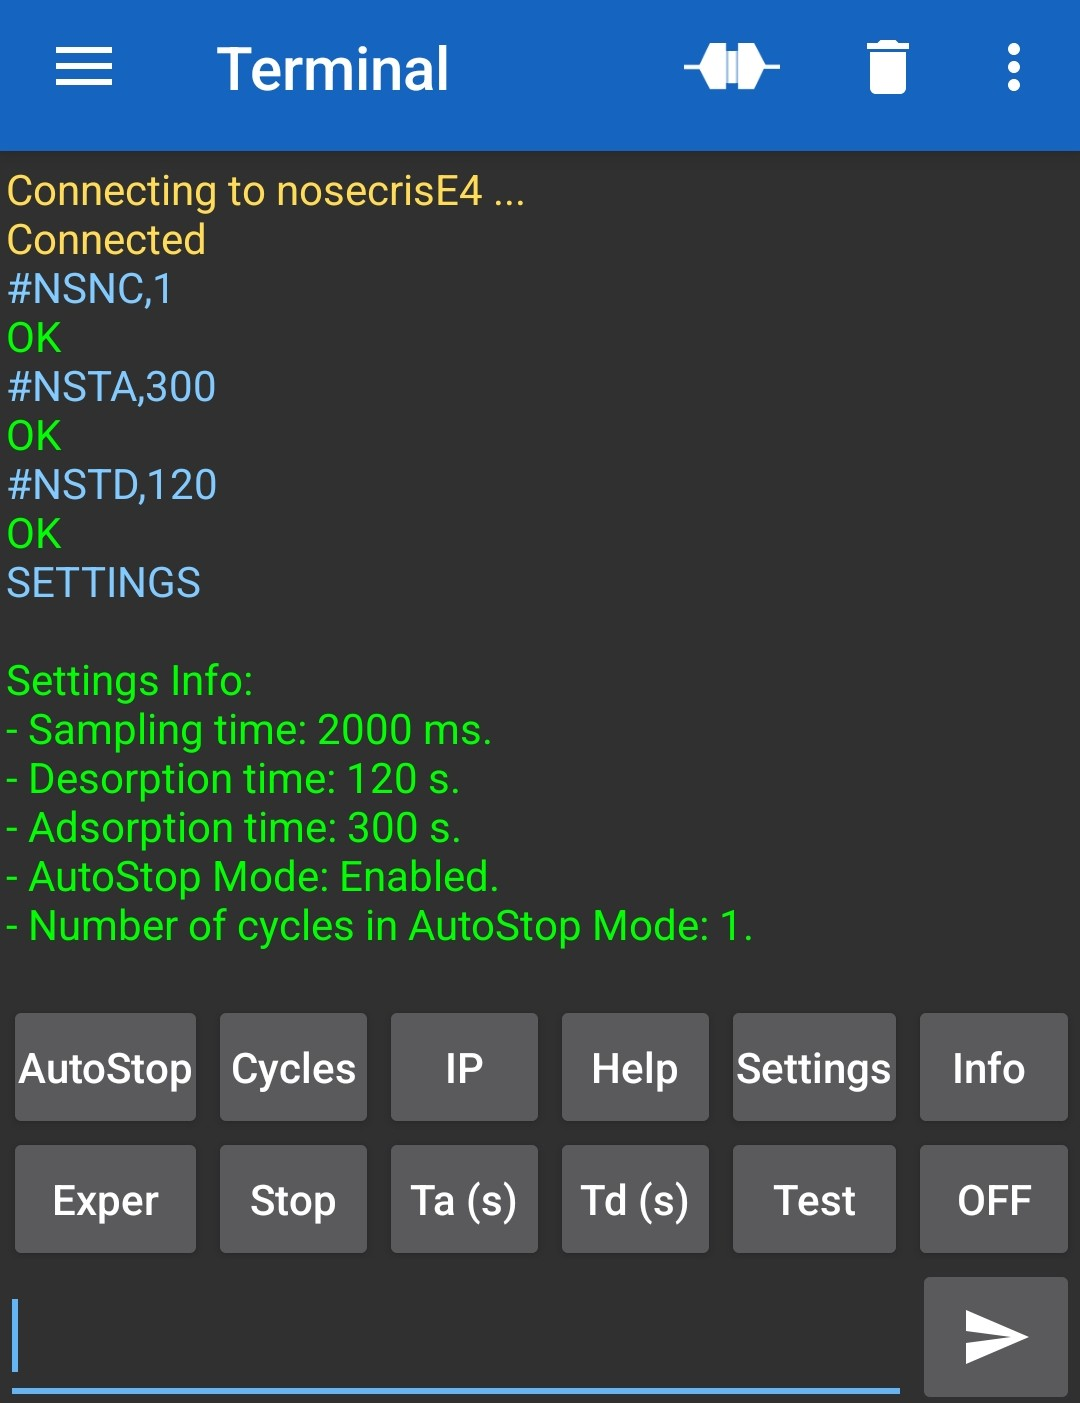
\includegraphics[width=0.4\textwidth]{pictures/InterfazBT1.jpg}
    \caption{Interfaz de la a plicación móvil para el control de la toma de muestras.}\label{fig:app_toma_muestras}
\end{figure}

\subsubsection{Limpieza del dataset}
Para la limpieza y preprocesamiento de los datos obtenidos durante la fase de toma de muestras, se busca crear un script que automatice este proceso y facilite la preparación del dataset para su posterior análisis y entrenamiento de la ANN\@. Existen varias posibilidades para llevar a cabo esta tarea, entre las que se incluyen:

\begin{itemize}
    \item \textbf{Python:}
    \begin{itemize}
        \item Cuenta con librerias como NumPy, Pandas, Matplotlib o Polaras para el procesamiento y visualización de datos.
        \item Sencillo de aprender y utilizar.
        \item Amplia comunidad y soporte.
        \item Limpieza reproducible.
        \item Familiaridad con el lenguaje.
    \end{itemize}
    \item \textbf{R:}
    \begin{itemize}
        \item Limpieza reproducible.
        \item Muy usado en investigación.
    \end{itemize}
    \item \textbf{Bash + herramientas UNIX:}
    \begin{itemize}
        \item Potente para archivos de texto.
        \item Muy rápido.
        \item Limpieza reproducible.
        \item Cero dependencias.
    \end{itemize}
    \item \textbf{SQL + scripts:}
    \begin{itemize}
        \item Exportación muy limpia.
        \item Limpieza reproducible.
    \end{itemize}
    \item \textbf{Apache Spark:}
    \begin{itemize}
        \item Escalable.
        \item Limpieza reproducible.
        \item Muy usado en entornos de investigación grandes.
    \end{itemize}
\end{itemize}

Dado que se trata de un script sencillo, que no tienen que procesar una gran cantidad de datos, se ha optado por utilizar Python para la limpieza de dichos datos. Esta elección se basa en la familiaridad con el lenguaje, la disponibilidad de librerías especializadas y la facilidad para crear scripts reproducibles que faciliten el análisis posterior.

\subsubsection{Entrenamiento de la ANN}
% Aquí se hablará de que se ha uasdo google colab y python porque el portatil no daba para más.

\subsubsection{Aplicación Bluetooth}